%!TEX TS-program = xelatex
%%%%%%%%%%%%%%%%%%%%%%%%%%%%%%%%%%%%%%%%%
% Friggeri Resume/CV for A4 paper format
% XeLaTeX Template
% Version 1.1
%
% A4 version author:
% Marvin Frommhold (depressiverobot.com)
% https://github.com/depressiveRobot/friggeri-cv-a4
%
% Original author:
% Adrien Friggeri (adrien@friggeri.net)
% https://github.com/afriggeri/CV
%
% License:
% CC BY-NC-SA 3.0 (http://creativecommons.org/licenses/by-nc-sa/3.0/)
%
% Important notes:
% This template needs to be compiled with XeLaTeX and the bibliography, if used,
% needs to be compiled with biber rather than bibtex.
%
%%%%%%%%%%%%%%%%%%%%%%%%%%%%%%%%%%%%%%%%%

% Options
% 'print': remove colors from this template for printing
% 'nocolors' to disable colors in section headers
\documentclass[nocolors]{friggeri-cv-a4}


\addbibresource{bibliography.bib} % Specify the bibliography file to include publications

\begin{document}

\header{Alcemir }{Rodrigues Santos}{Compuer Science Assistant Professor} % Your name and current job title/field

%----------------------------------------------------------------------------------------
% SIDEBAR SECTION
%----------------------------------------------------------------------------------------

\begin{aside} % In the aside, each new line forces a line break


\includegraphics[scale=0.5]{img/profile2.png}
~
 \section{Address}
 Teresina - Piau\'{i}
 Brazil
 ~
 \section{Tel \& Skype}
 +55 86  99851 3193
 alcemir\_santos
 ~
 \section{Mail}
 \href{mailto:alcemir@prp.uespi.br}{alcemir@prp.uespi.br}
 ~
 \section{Web \& Git}
 \href{https://www.alcemirsantos.com.br}{alcemirsantos.com.br}
 \href{https://github.com/alcemirsantos}{alcemirsantos@github}
~
 % use  \hspace{} or \vspace{} to change bubble size, if needed
 \section{Programming}
  Java 
\includegraphics[scale=0.40]{img/4stars.png}
  Flutter 
\includegraphics[scale=0.40]{img/3stars.png} 
  Python 
\includegraphics[scale=0.40]{img/2stars.png}
 ~
 \section{Personal Skills}
 {\color{red} $\varheartsuit$}Team Player,
 	Initiative,
 	Curiosity,
 	Problem Solving,
 	% \textbf{\vspace{2mm}Manage\vspace{2mm}},
 	Organized
 ~
\end{aside}

%----------------------------------------------------------------------------------------
% EDUCATION SECTION
%----------------------------------------------------------------------------------------
\section{Education}
\begin{entrylist}
	\entry
	{2014 - 2017}
	{Ph.D in Computer Science}
	{Federal University of Bahia}
	{4 years scholarship grant from FAPESB.\\}
	\entry
	{2011 - 2013}
	{Master's Degree in Computer Science}
	{Federal University of Minas Gerais}
	{2 years scholarship grant from CNPq.\\}
	\entry
	{2006 - 2010}
	{Bachelor's Degree in Computer Science}
	{Federal University of Piauí}
	{2$^{nd}$ Best grade among the classmates.\\}
	\entry
	{2003 - 2005}
	{High School Diploma}
	{CEBRAPI}
	{3$^{rd}$ Best grade among the classmates.}
\end{entrylist}

\section{Experience}
\begin{entrylist}
	 \entry
	{Oct 2018 \\ \~{}now}
	{Assistant Professor}
	{State University of Piau\'{i} - UESPI}
	{Since October 2018, I am working as a computer science assistant professor in this university. I teach graduation courses mainly in the topic of Software Engineering, such as \textit{(i)} Sofware Enginering; \textit{(ii)} Object Oriented Programming; \textit{(iii)} Analysis and Design of Object-oriented Software; \textit{(iv)} Enterpreneurship. Since mid-2019 I am the head of a computer science bachelor degree here.}
	\entry
	{Aug 2019\\\~{}Dec 2020}
	{Lecturer}
	{CEV Institute for Higher Education - iCEV}
	{During one year and a half, I worked as a sofware engineering degree lecturer in this college. I taught graduation courses such as \textit{(i)} Sofware Enginering and \textit{(ii)} Object-Oriented Programming; Analysis and Design of Object-oriented Software}
	\entry
	{Aug 2017\\\~{}Sep 2018}
	{Lecturer}
	{Federal University of Piau\'{i} - UFPI}
	{I worked at UFPI as a temporary lecturer for the Information Systems Bachelor Program. I have taught the following courses: \textit{(i)} Project and Development of Information Systems; \textit{(ii)} Analysis and Design of Object-oriented Software; \textit{(iii)} Logical Programming; \textit{(iv)} Object Oriented Programming.}
	\entry
	{Aug 2015 \\\~{}Jul 2016}
	{Visiting Scholar}
	{Universit\"at Passau}
	{I lived one year in Passau. During this time I had to work together with other \textit{Ph.D.} students from the University of Passau research group under supervision of Prof. Sven Apel. Among my responsabilities were to build a tool for collecting software repositories metadata about software conflicting merges and built the network from those developers who contributed to the conflicting merge. Most of the time I programmed with \texttt{Java} and \texttt{MySQL}, but also learned some \texttt{Python} and \texttt{R}. }
	\entry
	{2016}
	{Open-souce Software Sporadic Contributor}
	{JGit}
	{During my time at the Unviversity of Passau I have contributed some pieces of code, including test cases, to the open-source \texttt{JGit} community.  JGit is a pure Java library implementing the Git version control system.}
\end{entrylist}
\newpage
\begin{entrylist}
	\entry
	{2013 - 2014}
	{Research Assistent}
	{Reuse in Software Engineering Laboratory (RiSE Labs)}
	{During one year I had to work together with the \textit{Master} and \textit{Ph.D.} students from the research group. Among my responsabilities were to help the students with the design and execution of software engineering experiments in different Software Engineering topics, as well as sofware development and testing with \texttt{Java} and \texttt{Objective-C}. \\}
	\entry
	{01/2010-02/2011}
	{Web Developer}
	{Freelance}
	{Just prior to finish my CS Degree I have worked as Full-Stack Freelance Web-developer in small projects for local events and our local Judo team with \texttt{PHP}.\\}
	\entry
	{2008 - 2009}
	{Research Internship}
	{Federal University of Piauí}
	{During one year I have programmed neural networks addressing interger optimization problems mainly using SciLab.}
	
\end{entrylist}

\begin{aside}
	 ~
	\section{Publications}
	\href{https://dblp.org/pid/88/10587.html}{DBLP}
	\href{https://scholar.google.com.br/citations?user=\_CgZOX0AAAAJ}{Google Scholar}
	~
	\section{OS Preference}
	\textbf{MacOS}
\includegraphics[scale=0.40]{img/5stars.png}
	\textbf{GNU/Linux}
\includegraphics[scale=0.40]{img/4stars.png}
	\textbf{Windows}
\includegraphics[scale=0.40]{img/1stars.png}
	~
	\section{Places Lived}
	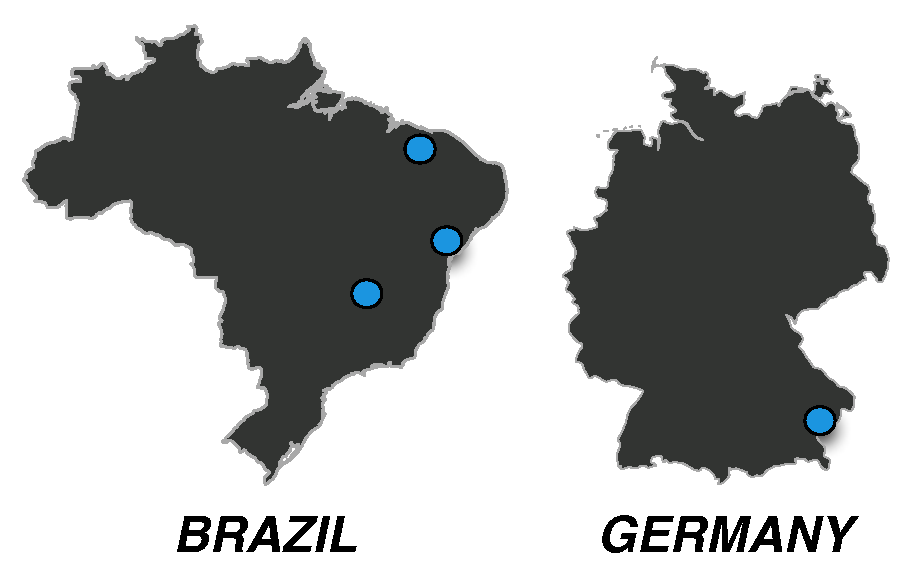
\includegraphics[scale=0.25]{img/places.pdf}
	~
	\section{Languages}
	\textbf{Portuguese}
\includegraphics[scale=0.40]{img/5stars.png}
	\textbf{English}
\includegraphics[scale=0.40]{img/4stars.png}
	\textbf{German}
\includegraphics[scale=0.40]{img/3stars.png}
	\textbf{Spanish}
\includegraphics[scale=0.40]{img/1stars.png}
	~
\end{aside}

\section{Publications}

\includegraphics[scale=.15]{img/star.pdf}~ This star indicates the ones I consider the most relevant ones.
 
\subsection{in Journals}

\includegraphics[scale=.15]{img/star.pdf}~VALE, G.; SCHMID, A.; \textbf{SANTOS, A. R.};  ALMEIDA, E. S..; APEL, S.\\
\textbf{On the Relation Between GitHub Communication Activity and Merge Conflicts.} \\
\emph{Empirical Software Engineering 25, 402–433 (2020)}.\\ \url{https://doi.org/10.1007/s10664-019-09774-x}


\includegraphics[scale=.15]{img/star.pdf}~\textbf{SANTOS, A. R.}; MACHADO, I. C. ; ALMEIDA, E. S..; SIEGMUND, J.; APEL,S.\\
\textbf{Comparing the Influence of Using Feature-Oriented Programming and Conditional Compilation on Comprehending Feature-Oriented Software.} \\
\emph{Empirical Software Engineering. 24, 1226–1258 (2019).}\\ \url{https://doi.org/10.1007/s10664-018-9658-x}.

CARVALHO, M. L. L.; SILVA, M. L. G.; GOMES, G. S. S.; \textbf{SANTOS, A. R.}; MACHADO, I. C.; SOUZA, M. L. J.; ALMEIDA, E. S..\\
\textbf{On the implementation of dynamic software product lines: An exploratory study}.\\
\emph{Journal of Systems and Software. 136: 74-100 (2018).} \\
\url{https://doi.org/10.1016/j.jss.2017.11.004}\\


\includegraphics[scale=0.15]{img/star.pdf}~OLIVEIRA, R. P. ; \textbf{SANTOS, A. R.} ; GOMES, G.; ALMEIDA, E. S..\\
\textbf{Evaluating Lehman's Laws of Software Evolution within Software Product Lines Industrial Projects.}\\
\emph{Journal of Systems and Software. Volume 131. 347--365 (2017).}\\
\url{https://doi.org/10.1016/j.jss.2016.07.038}.\\

\textbf{SANTOS, A. R.} ; ALMEIDA, E. S.. \\
\textbf{Do \#ifdef-based Variation Points Realize Feature Model Constraints?}\\
\emph{Software Engineering Notes , v. 40, p. 1-5, 2015.}\\


\subsection{in Conferences}

\textbf{SANTOS, A. R.}; MACHADO, I. C. ; ALMEIDA, E. S..\\
\textbf{Aspects Influencing Feature-Oriented Software Comprehension: Observations from a Focus Group.} \\
\emph{Proceedings of the 11$^{th}$ Brazilian Symposium on Components, Architecture, and Reuse (SBCARS). Fortaleza, 2017. p. 1-10.}\\


\includegraphics[scale=.15]{img/star.pdf}~\textbf{SANTOS, A. R.} ; MACHADO, I. C. ; ALMEIDA, E. S..\\ 
\textbf{RiPLE-HC: JavaScript Systems Meets SPL Composition.}\\
\emph{Proceedings of the 20$^{th}$ Software Product Lines Conference (SPLC). Beijing. p. 154-163. (2016).}\\
 \url{https://doi.org/10.1145/2934466.2934486}.\\

\textbf{SANTOS, A. R.}; MACHADO, I. C. ; ALMEIDA, E. S..\\
\textbf{RiPLE-HC: Visual Support for Features Scattering and Interactions.} \\
\emph{Proceedings of the 20$^{th}$ Software Product Lines Conference. Beijing, 2016. p. 320-323.}\\

SOUZA, M. L. J. ; \textbf{SANTOS, A. R.} ; MACHADO, I. C. ; GOMES, G. ; ALMEIDA, E. S..\\
\textbf{Evaluating Variability Modeling Techniques for Dynamic Software Product Lines: A Controlled Experiment.} \\
\emph{Proceedings of the 10$^{th}$ Brazilian Symposium on Components, Architecture, and Reuse (SBCARS). Londrina, 2016. p. 1-10.}\\

SANTOS, J. A. M. ; \textbf{SANTOS, A. R.}; MENDON\c{C}A, M.. \\
\textbf{Investigating bias in the search phase of Software Engineering secondary studies.} \\
\emph{12$^{th}$ Workshop on Experimental Software Engineering. \\
	Proceedings of 18$^{th}$ Ibero-American Conference on Software Engineering (CiBSE), 2015.}\\


\includegraphics[scale=.15]{img/star.pdf}~ \textbf{SANTOS, A. R.}  ; DE OLIVEIRA, R. P.; DE ALMEIDA, E. S..\\
\textbf{Strategies for consistency checking on software product lines.}\\
\emph{Proceedings of the 19$^{th}$ International Conference on Evaluation and Assessment in Software Engineering (EASE). Nanjing.  p. 1-14. (2015).}\\
\url{https://doi.org/10.1145/2745802.2745806}.\\

SOUZA, M. L. J. ; \textbf{SANTOS, A. R.}  ; ALMEIDA, E. S.. \\
\textbf{Towards the Selection of Modeling Techniques for Dynamic Software Product Lines.} \\
\emph{Proceedings of the 5$^{th}$ International Workshop on Product Line Approaches in Software Engineering (PLEASE). Florence, 2015. p. 19-22. }\\

\textbf{SANTOS, A. R.}  ; FARIAS, M. A. F. ; ALMEIDA, E. S. ; MENDONCA, M. ; SANTANNA, C. N..\\ 
\textbf{How developers deal with Code Smells: the case of the SourceMiner Evolution team.} \\
\emph{Workshop on Software Visualization, Evolution and Maintenance (VEM).
	Proceedings of the 5$^{th}$ Brazilian Conference on Software: Theory and Practice (CBSoft). Maceió, 2014. p. 1-6.}\\

VALE, T; CABRAL, B.; ALVIM, L; SOARES, L. ; \textbf{SANTOS, A. R.} ; MACHADO, I.; SOUZA, I.; FREITAS, I.; ALMEIDA, E..\\
\textbf{SPLICE: A Lightweight Software Product Line Development Process for Small and Medium Size Projects.} \\
\emph{Proceedings of the 8$^{th}$ Brazilian Symposium on Software Components, Architectures, and Reuse (SBCARS). Maceió, 2014. p. 42-52.}\\


\includegraphics[scale=.15]{img/star.pdf}~\textbf{SANTOS, A. R.}  ; GAIA, F. N. ; FIGUEIREDO, E. ; SANTOS NETO, P. ; ARAUJO, J..\\
\textbf{Test-based SPL extraction: an exploratory study.} \\
\emph{Proceedings of the ACM Symposium on Applied Computing (SAC). Coimbra, 2013. p. 1031-1036.}\\

SANTOS, I. S. ; \textbf{SANTOS, A. R.}  ; SANTOS NETO, P..\\
\textbf{Reusing Functional Testing in order to Decrease Performance and Stress Testing Costs.}\\
\emph{Proceedings of the 23$^{rd}$ International Conference on Software Engineering and Knowledge Engineering (SEKE). Miami, 2011. p. 1-5.}\\

ALVES, P. ; \textbf{SANTOS, A. R.}  ; FIGUEIREDO, E. ; FERRARI, F..\\
\textbf{How do Programmers Learn AOP? An Exploratory Study of Recurring Mistakes.} \\
\emph{5$^{th}$ Latin-American Workshop on Aspect-Oriented Software Development (LA-WASP).\\
	Proceedings of the 2$^{nd}$ Brazilian Conference on Software: Theory and Practice (CBSoft). São Paulo, 2011.}\\

\section{Honors \& Awards}
\begin{entrylist}
	\entry
	{2014}
	{Among Best Papers}
	{VaMoS Workshop}
	{8th International Workshop on Variability Modelling of Software-intensive Systems}\\
	
	\entry
	{2013}
	{Student Travel Award}
	{ACM SAC Conference}
	{SIGAPP Student Travel Award Program of the Association of Computing Machinery (ACM).}\\
\end{entrylist}

\section{Certifications}
\begin{entrylist}
	\entry
	{2014}
	{English Proficience Level B2}
	{TOEFL ITP}\\
	
	\entry
	{2016}
	{German Proficience Level B2}
	{Volkshochschule Passau}\\
\end{entrylist}



%----------------------------------------------------------------------------------------
% INTERESTS SECTION
%----------------------------------------------------------------------------------------

\section{Interests}
\begin{description}
	\item[Professional:] empirical sofware engineering; software maintenance and evolution; enterpreneurship.
	
	\item[Personal:] guitar; music; judo.
\end{description}


%----------------------------------------------------------------------------------------
% PUBLICATIONS SECTION
%----------------------------------------------------------------------------------------

%----------------------------------------------------------------------------------------
\hspace{4cm}
\begin{flushleft}
	\emph{\today}
\end{flushleft}
\begin{flushright}
	\emph{Alcemir Rodrigues Santos}
\end{flushright}


\newpage
\section{List of names for reference}
\vspace{2cm}
\begin{entrylist}
	\entry
	{iCEV}
	{Prof. Dr. Fábbio Anderson Silva Borges}
	{SE Degree Head}
	{\href{mailto:fabbioborges@grupocev.com}{fabbioborges@grupocev.com}}\\
	
	\entry
	{UFBA}
	{Prof. Dr. Eduardo Santanta de Almeida}
	{Ph.D. Advisor}
	{\href{mailto:esa@dcc.ufba.br}{esa@dcc.ufba.br}}\\
	
	\entry
	{UFBA}
	{Prof. Dr. Ivan do Carmo Machado}
	{Ph.D. Co-advisor}
	{\href{mailto:ivanmachado@dcc.ufba.br}{ivanmachado@dcc.ufba.br}}\\
	
	\entry
	{Saarland University}
	{Prof. Dr. Sven Apel}
	{Passau University Host}
	{\href{mailto:apel@cs.uni-saarland.de}{apel@cs.uni-saarland.de}}\\
	
	\entry
	{UFMG}
	{Prof. Dr. Eduardo Figueiredo}
	{M.Sc. Advisor}
	{\href{mailto:figueiredo@dcc.ufmg.br}{figueiredo@dcc.ufmg.br}}\\
	
	\entry
	{UFPI}
	{Prof. Dr. Pedro de Alcântara dos Santos Neto}
	{M.Sc. Co-advisor}
	{\href{mailto:pasn@ufpi.edu.br}{pasn@ufpi.edu.br}}\\		
	
	
\end{entrylist}


\end{document}
